% \usepackage{listings}
% \usepackage{graphicx, color}
% その他設定がmain.texにあります

\section{実際のオンラインジャッジシステムの活用例}

OJSの活用例として, 競技プログラミングサイトAtCoder\cite{AtCoder}を紹介する. 

\subsection{AtCoderとは}

AtCoderは, 「競技プログラミング」と呼ばれるコンテストを行うサービスである. 
日本国内の競技プログラミングコンテストサイトとしては最大規模であり, 日本人登録者が16万人, 海外を含め30万人以上の登録者がいる. 
また, 毎週コンテストが開催されており, 8,000人以上が参加している. 

プログラミング言語はC言語, C++, Java, Python3, Rustを始めとした40以上の言語に対応しており, 参加者は好きな言語を利用してコンテストに参加することができる. 

\subsection{競技プログラミングとは}
競技プログラミングは, 様々なアルゴリズムや数学的知識を利用し, 与えられた問題に適するプログラムを提出する速度を競うコンテストである. 

AtCoderにおいては, コンテストで与えられる問題にそれぞれ得点が決まっており, 問題に正解することで得点を得ることができる. 
そして, 開催時間内に得た得点及びその提出時間により順位が決定される. 
誤ったプログラムを提出すると, 1回につき提出時間に5分のペナルティが追加されるため, より速く, 正確にプログラミングを行うことが重要となる. 

\subsection{AtCoderのコンテスト}
AtCoderにおける定期開催コンテストは4種類あり, 表\ref{tab:atcoder contest}のようになっている. 
ABC, ARC, AGCでは入出力が予め決まっており, プログラムを提出することにより正誤判定が行われる. 
AHCのみヒューリスティックと呼ばれる形式であり, 最適解を求めることが難しい問題に対しより最適解に近い値を求めることを目的とするコンテストである. 

コンテストではそれぞれの問題に対してサンプルとして1つから3つのテストケースが公開されており, ユーザーはこのテストケースを利用し, AtCoder上のコードテストページや自分の開発環境でテストを行うことができる. 

\begin{table}[H]
    \caption{AtCoderの定期開催コンテスト}
    \label{tab:atcoder contest}
    \centering

    \begin{tabular}{|l||l|l|l|}
        \hline
        コンテスト名 & 難易度 & 時間 & 問題数 \\ \hline
        \hline
        AtCoder Beginner Contest(ABC) & 初心者~中級者向け & 100分 & 8問 \\ \hline
        AtCoder Regular Contest(ARC) & 初心者~上級者向け & 120分 & 6問 \\ \hline
        AtCoder Grand Contest(AGC) & 中級者~上級者向け & 150~180分 & 6問 \\ \hline
        AtCoder Heuristic Contest(AHC) & 初心者~上級者向け & 240~480分 & 1問 \\ \hline
        
    \end{tabular}

\end{table}

\subsection{AtCoderにおけるオンラインジャッジシステムの利用}

AtCoderでは, 提出されたプログラムはOJSを利用し, 計算時間, メモリ使用量のそれぞれの制限内で処理が終わっているか, および出力結果が正しいかを判断したうえで正誤判定が行われる. 
誤ったプログラムを提出した場合, CE(Compilation Error, コンパイルエラー), RE(Runtime Error, 実行時エラー), TLE(Time Limit Exceeded, 制限時間超過), WA (Wrong Answer, 出力結果が誤っている)など, どのような理由で間違っているのかが表示される. 

\clearpage

\subsection{オンラインジャッジシステムによる実行例}

AtCoderので2022年1月8日に行われたコンテスト, AtCoder Beginner Contest 234(ABC234)の過去問から, B問題を解いた場合の状況を例に挙げる. 
ABC234では, A~G, Exの8問の問題が出題された. 
問題の難易度はA問題が一番易しく, Ex問題が一番難しくなっており, B問題は2番目に易しい問題である. 

ABC234のB問題は以下のような問題となる. 

\begin{itembox}[l]{B - Longest Segment}
\textbf{問題文}

二次元平面上に$ N $個の点があります. $i$個目の点の座標は ($x_i$, $y_i$) です. 

この中から2個の点を選ぶとき, それらを結ぶ線分の長さの最大値を求めてください. 
\\

\textbf{制約}

・実行時間制限:2sec

・メモリ制限:1024MB

・2 $\leq$ $N$ $\leq$ 100

・-1000 $\leq$ $x_i, y_i$ $\leq$ 1000

・ ($x_i, y_i$) \neq ($x_j, y_j$) ($i \neq j$)

・入力はすべて整数
\\

\textbf{入力}

入力は以下の形式で標準入力から与えられる. 

$N$ \\ $x_1 y_1$ \\ $x_2 y_2$ \\ : \\ $x_N y_N$
\\

\textbf{出力}

2点を結ぶ線分の長さの最大値を出力せよ. 

想定解との絶対誤差または相対誤差が$10^{-6}$以下であれば正解とみなされる. 


\end{itembox}
% これ, 図にしたほうがいいのかしら?


\clearpage

例として, 問題に対して提出したコードを時系列順に図\ref{code:wa1}, 図\ref{code:wa2}, 図\ref{code:ac}に示す. 
また, それぞれの提出結果を図\ref{code:wa1-sub}, 図\ref{code:wa2-sub}, 図\ref{code:ac-sub}に示す. 

図\ref{code:wa1}のコードには2点の問題があり, 配列の参照エラーと計算ミスがある. 
このコードを提出した結果, 図\ref{code:wa1-sub}のように実行時エラーが発生した. 


\begin{figure}[H]
    \centering
\begin{lstlisting}[style = customPy]
#!/usr/bin/env python3

N = int(input())
XY = [list(map(int, input().split())) for _ in range(N)]

ans = 0

for i in range(N):
    // 配列外の数値を参照している
    for j in range(i + 1, N + 1):
        lx = XY[i][0]; ly = XY[i][1]
        rx = XY[j][0]; ry = XY[j][1]
        ans = max(ans, (rx - lx) ** 2 + (ry - ly) ** 2)

print(ans)
\end{lstlisting}

\caption{配列参照を誤った提出コード}
    \label{code:wa1}
\end{figure}

\begin{figure}[H]
    \centering
    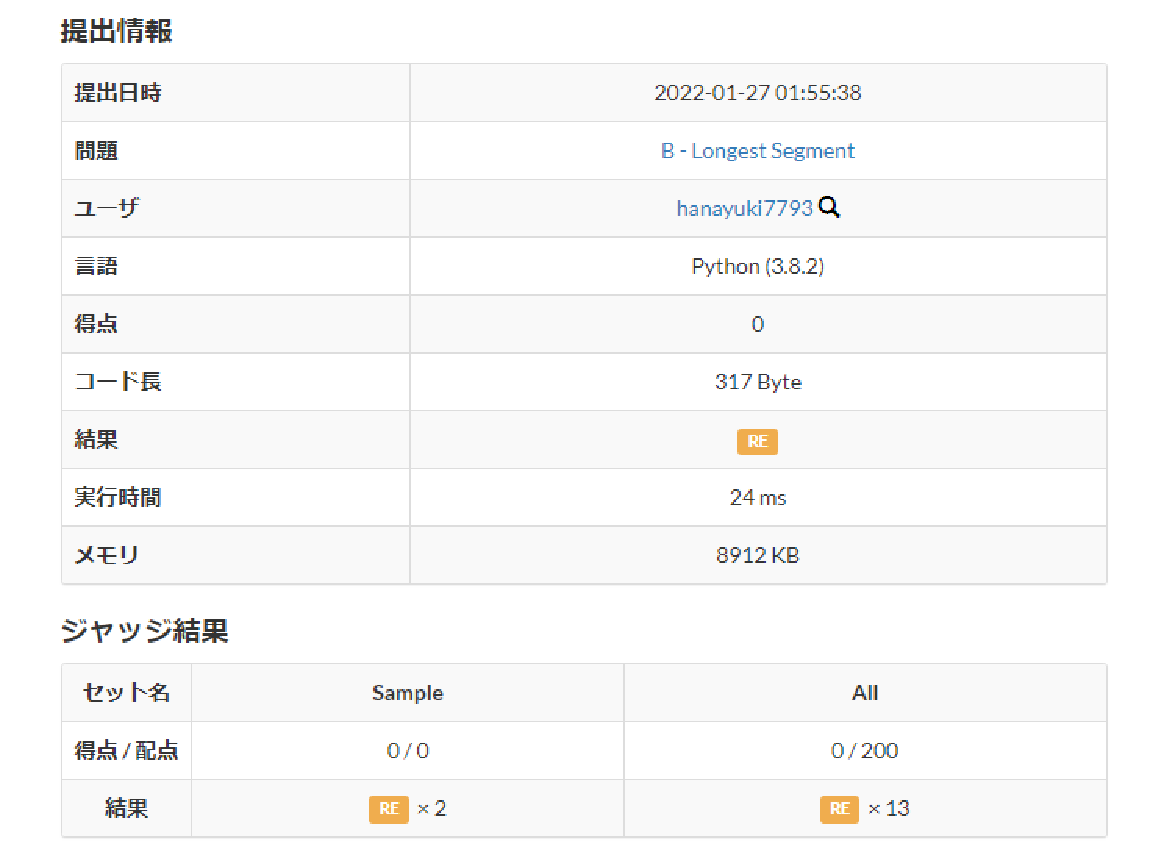
\includegraphics[width=0.95\linewidth, clip]{wa1.pdf}
    \caption{配列参照を誤った提出コードの提出結果}
    \label{code:wa1-sub}
\end{figure}

\clearpage

ソースコードを確認すると, 10行目で要素数がNの配列XYに対し, 添字Nでアクセスすることにより配列の参照エラーが発生していた. 
そこで, 8行目のNをN-1に, 10行目のN+1をNに変更し図\ref{code:wa2}のコードを提出した. 
提出した結果, 図\ref{code:wa2-sub}のように計算結果が誤っていることが分かった. 

\begin{figure}[H]
    \centering
\begin{lstlisting}[style = customPy]
#!/usr/bin/env python3

N = int(input())
XY = [list(map(int, input().split())) for _ in range(N)]

ans = 0

for i in range(N - 1):
    for j in range(i + 1, N):
        lx = XY[i][0]; ly = XY[i][1]
        rx = XY[j][0]; ry = XY[j][1]
        ans = max(ans, (rx - lx) ** 2 + (ry - ly) ** 2)

// 平方根を求め忘れている
print(ans)
\end{lstlisting}
\caption{計算を誤った提出コード}
    \label{code:wa2}
\end{figure}

\begin{figure}[H]
    \centering
    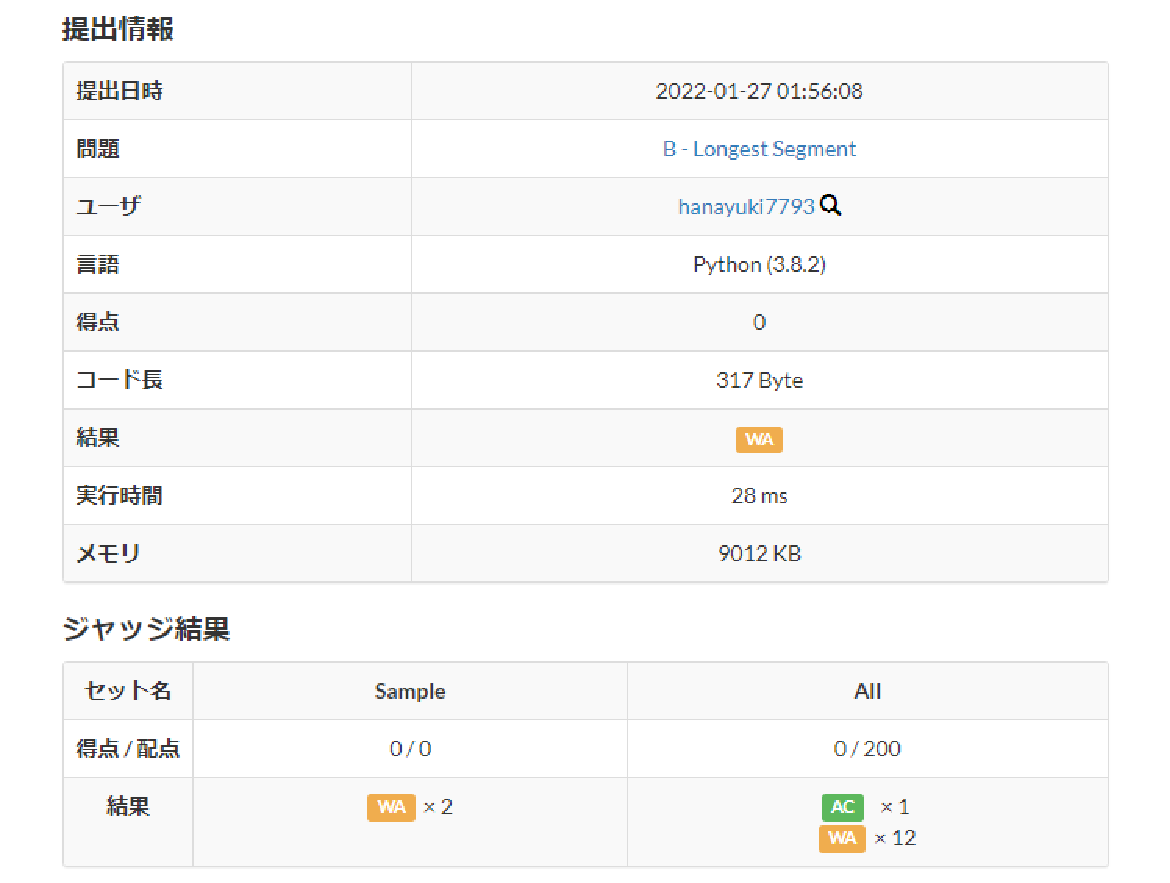
\includegraphics[width=0.95\linewidth, clip]{wa2.pdf}
    \caption{計算を誤った提出コードの提出結果}
    \label{code:wa2-sub}
\end{figure}

\clearpage
問題を確認すると, 2点を結ぶ線分の長さを求める問題となっており, 答えは平方根を取る必要があることが分かった. 
そこで, 15行目の計算の修正を行い図\ref{code:ac}のコードを提出した. 

\begin{figure}[H]
    \centering
\begin{lstlisting}[style = customPy]
#!/usr/bin/env python3

import math

N = int(input())
XY = [list(map(int, input().split())) for _ in range(N)]

ans = 0

for i in range(N - 1):
    for j in range(i + 1, N):
        lx = XY[i][0]; ly = XY[i][1]
        rx = XY[j][0]; ry = XY[j][1]
        ans = max(ans, (rx - lx) ** 2 + (ry - ly) ** 2)

print(math.sqrt(ans))

\end{lstlisting}
\caption{正しい提出コード}
    \label{code:ac}
\end{figure}

\begin{figure}[H]
    \centering
    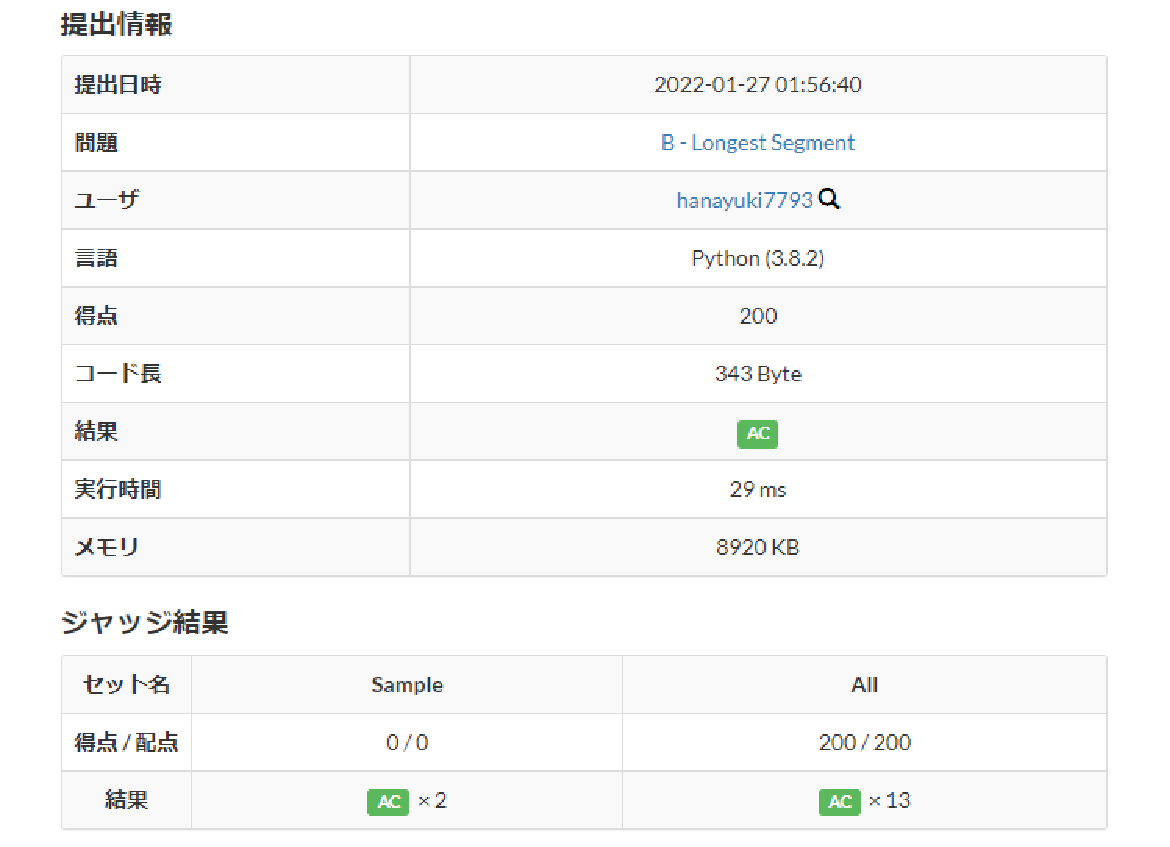
\includegraphics[width=0.95\linewidth, clip]{ac.pdf}
    \caption{正しい提出コードの提出結果}
    \label{code:ac-sub}
\end{figure}

\clearpage
以上のように, 提出結果を確認することによりどのようなエラーが発生しているかが分かり, それを手掛かりにデバッグを行うことができる. 
また, それまでの提出結果は図\ref{pic:all}のように全て参照することが出来るようになっており, 過去に提出したコードも確認することができる. 

\begin{figure}[H]
    \centering
    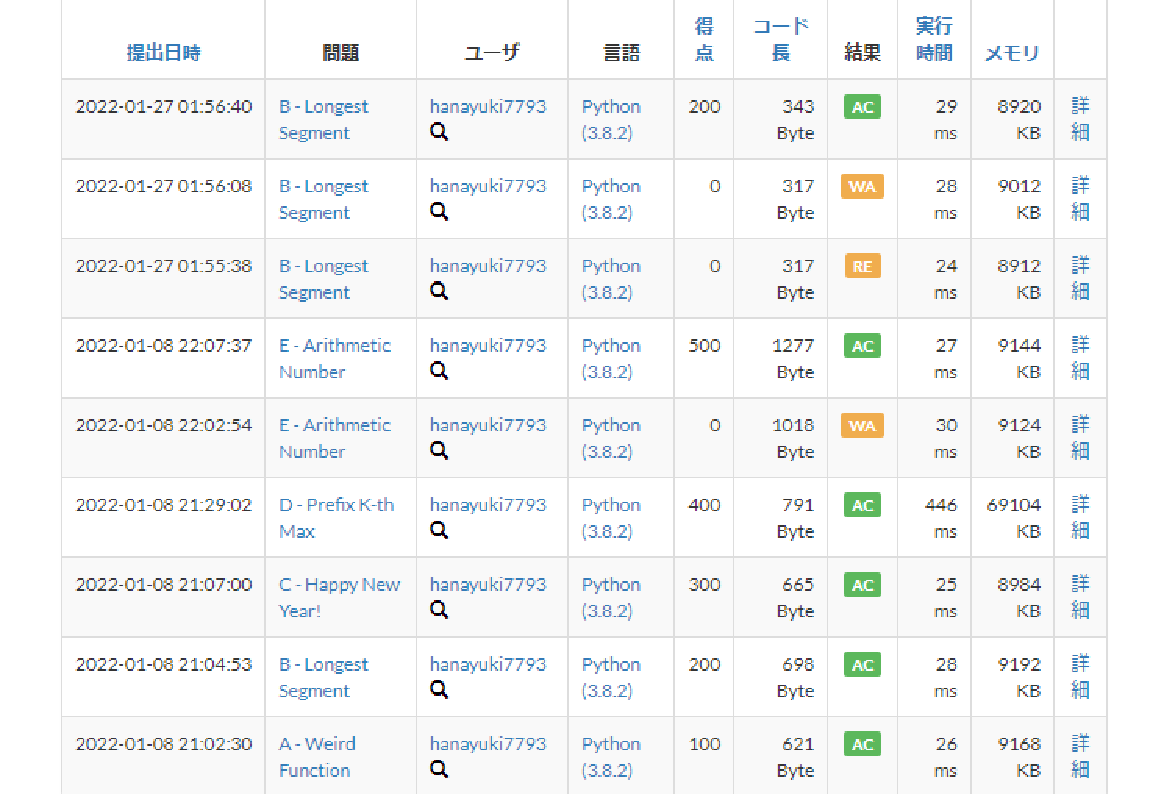
\includegraphics[width=0.95\linewidth, clip]{all2.pdf}
    \caption{提出履歴}
    \label{pic:all}
\end{figure}

